\let\negmedspace\undefined
\let\negthickspace\undefined
\documentclass[journal]{IEEEtran}
\usepackage[a5paper, margin=10mm, onecolumn]{geometry}
\usepackage{tfrupee} % Include tfrupee package

\setlength{\headheight}{1cm} 
\setlength{\headsep}{0mm}     

\usepackage{gvv-book}
\usepackage{gvv}
\usepackage{cite}
\usepackage{amsmath,amssymb,amsfonts,amsthm}
\usepackage{algorithmic}
\usepackage{graphicx}
\usepackage{textcomp}
\usepackage{xcolor}
\usepackage{txfonts}
\usepackage{listings}
\usepackage{enumitem}
\usepackage{mathtools}
\usepackage{gensymb}
\usepackage{comment}
\usepackage[breaklinks=true]{hyperref}
\usepackage{tkz-euclide} 
\usepackage{listings}
\def\inputGnumericTable{}                                 
\usepackage[latin1]{inputenc}                                
\usepackage{color}                                            
\usepackage{array}                                            
\usepackage{longtable}                                       
\usepackage{calc}                                             
\usepackage{multirow}                                         
\usepackage{hhline}                                           
\usepackage{ifthen}                                           
\usepackage{lscape}
\usepackage{circuitikz}
\tikzstyle{block} = [rectangle, draw, fill=blue!20, 
    text width=4em, text centered, rounded corners, minimum height=3em]
\tikzstyle{sum} = [draw, fill=blue!10, circle, minimum size=1cm, node distance=1.5cm]
\tikzstyle{input} = [coordinate]
\tikzstyle{output} = [coordinate]


\begin{document}

\bibliographystyle{IEEEtran}
\vspace{3cm}

\title{8.3.16}
\author{AI25BTECH11036-SNEHAMRUDULA}
 \maketitle
{\let\newpage\relax\maketitle}
\renewcommand{\thefigure}{\theenumi}
\renewcommand{\thetable}{\theenumi}
\setlength{\intextsep}{10pt} 
\numberwithin{equation}{enumi}
\numberwithin{figure}{enumi}
\renewcommand{\thetable}{\theenumi}
\textbf{Question:-}\;
An arch is in the form of a semi-ellipse. It is $8 \, \text{m}$ wide and $2 \, \text{m}$ high at the centre. Find the height of the arch at a point $1.5 \, \text{m}$ from one end?

\solution \\

We are given a semi-ellipse of width $8\,m$ and height $2\,m$ at the centre.
\subsection*{Step 1: Standard Form}
For an ellipse, the equation is
\begin{align}
\vec{q}^T\vec{V}\vec{q} = 1
\end{align}
where
\begin{align}
\vec{V} = \myvec{\frac{1}{a^2} & 0 \\ 0 & \frac{1}{b^2}}
\end{align}
Here, the semi-major axis $a = 4$ (half of 8 m) and semi-minor axis $b = 2$.

Thus,
\begin{align}
\vec{V} = \myvec{\frac{1}{16} & 0 \\ 0 & \frac{1}{4}}
\end{align}

\subsection*{Step 2: Equation of Ellipse}
Let 
\begin{align}
\vec{q} = \myvec{\alpha \\ \beta}
\end{align}
Substituting into (1),
\begin{align}
\frac{\alpha^2}{16} + \frac{\beta^2}{4} = 1
\end{align}

\subsection*{Step 3: Position at 1.5 m from End}
Since the width is $8\,m$, the end corresponds to $\alpha = \pm 4$.
At a point $1.5\,m$ from the end, the coordinate is
\begin{align}
\alpha = 4 - 1.5 = 2.5
\end{align}

\subsection*{Step 4: Solve for Height}
Substitute $\alpha = 2.5$ in (6):
\begin{align}
\frac{(2.5)^2}{16} + \frac{\beta^2}{4} = 1
\end{align}
\begin{align}
\frac{6.25}{16} + \frac{\beta^2}{4} = 1
\end{align}
\begin{align}
\frac{\beta^2}{4} = 1 - 0.390625
\end{align}
\begin{align}
\frac{\beta^2}{4} = 0.609375
\end{align}
\begin{align}
\beta^2 = 2.4375
\end{align}
\begin{align}
\beta \approx 1.561
\end{align}

\subsection*{Final Answer}
Hence, the height of the arch at a point $1.5\,m$ from the end is approximately
\begin{align}
\beta \approx 1.56 \, m
\end{align}
\begin{figure}[h!]
    \centering
    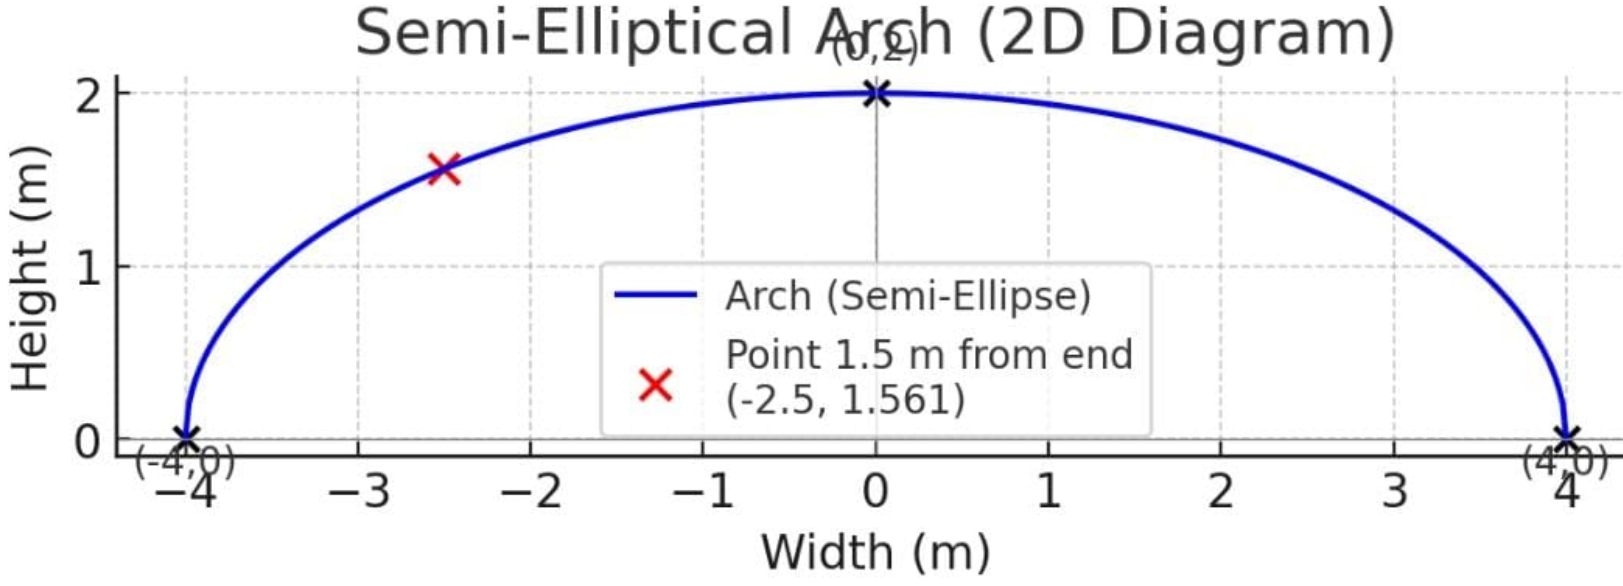
\includegraphics[height=0.2\textheight, keepaspectratio]{fig8.3.16.png}
    \label{figure_1}
\end{figure}
\end{document}